\documentclass[12pt,a4paper]{article}

\usepackage{polyglossia}
\setmainlanguage{french}

\usepackage{amsmath, amssymb}

\usepackage{graphicx}
\usepackage{caption}

\usepackage{siunitx} % Pour les unités

\usepackage{geometry}
\geometry{top=2cm, bottom=2.5cm, left=3cm, right=3cm}
\setlength{\parindent}{0pt}

\usepackage{enumitem}

\usepackage{hyperref}

\usepackage{xcolor}

\usepackage{multicol}
\setlength{\columnseprule}{1pt}
\def\columnseprulecolor{\color{gray}}

\usepackage{tcolorbox}


\usepackage{import}
\usepackage{xifthen}
\usepackage{pdfpages}
\usepackage{transparent}
\usepackage{float}

\newcommand{\incfig}[1]{%
	\def\svgwidth{\columnwidth}
	\import{./figures/}{#1.pdf_tex}
}


\newcommand{\RomanNum}[1] %pour les chiffre romain
{\MakeUppercase{\romannumeral #1}}


\usepackage{pdfpages}



\setmainfont{Arial}





\title{|}
\author{}
\date{\today}

\begin{document}

	
	
	\tableofcontents
	
	\newpage
	
	
	
	
	\section{Introduction générale}
	
	Le présent document s’inscrit dans le cadre du module Organisation de Chantier (ODC). Il a pour objectif de présenter l’organisation, la planification et la gestion des ressources nécessaires à la réalisation d’un immeuble en béton armé de type R+2, d’une surface de 500 m² par étage, soit une surface totale bâtie d’environ 1 500 m².
	
	\vspace{\baselineskip}
	
	Ce projet est traité comme un projet pédagogique, permettant d’appliquer les notions fondamentales de l’ODC telles que :
	
	
	\begin{itemize}
		\item Le découpage des travaux,
		\item la planification temporelle,
		\item l’affectation des ressources humaines et matérielles,
		\item l’estimation des coûts,
	\end{itemize}
	
	\vspace{\baselineskip}
	
	La planification du projet a été réalisée à l’aide du logiciel ProjectLibre, outil de gestion de projet open source, permettant d’élaborer un planning détaillé, d’affecter les ressources et d’estimer les coûts globaux du chantier.
	
	
	\section{Présentation du projet}
	
	
	\begin{itemize}
		\item Nature du projet : Construction d’un immeuble d’habitation
		
		\item Type de structure : Béton armé
		
		\item Nombre de niveaux : Rez-de-chaussée + 2 étages (R+2)
		
		\item Surface par étage : 500 m²
		
		\item Surface totale construite : 1 500 m²
		
		\item Fondations : Béton armé (semelles isolées)
		
		\item Système porteur : Portiques.
	\end{itemize}
	
	
	\section{Découpage du projet}
	
	Le projet a été décomposé en grandes phases, chacune subdivisée en tâches et sous-tâches dans ProjectLibre : \textbf{\underline{(voir le fichier du projet)}}
	
	\begin{figure}[H]
		\centering
		\caption{Tableau des tâches}
		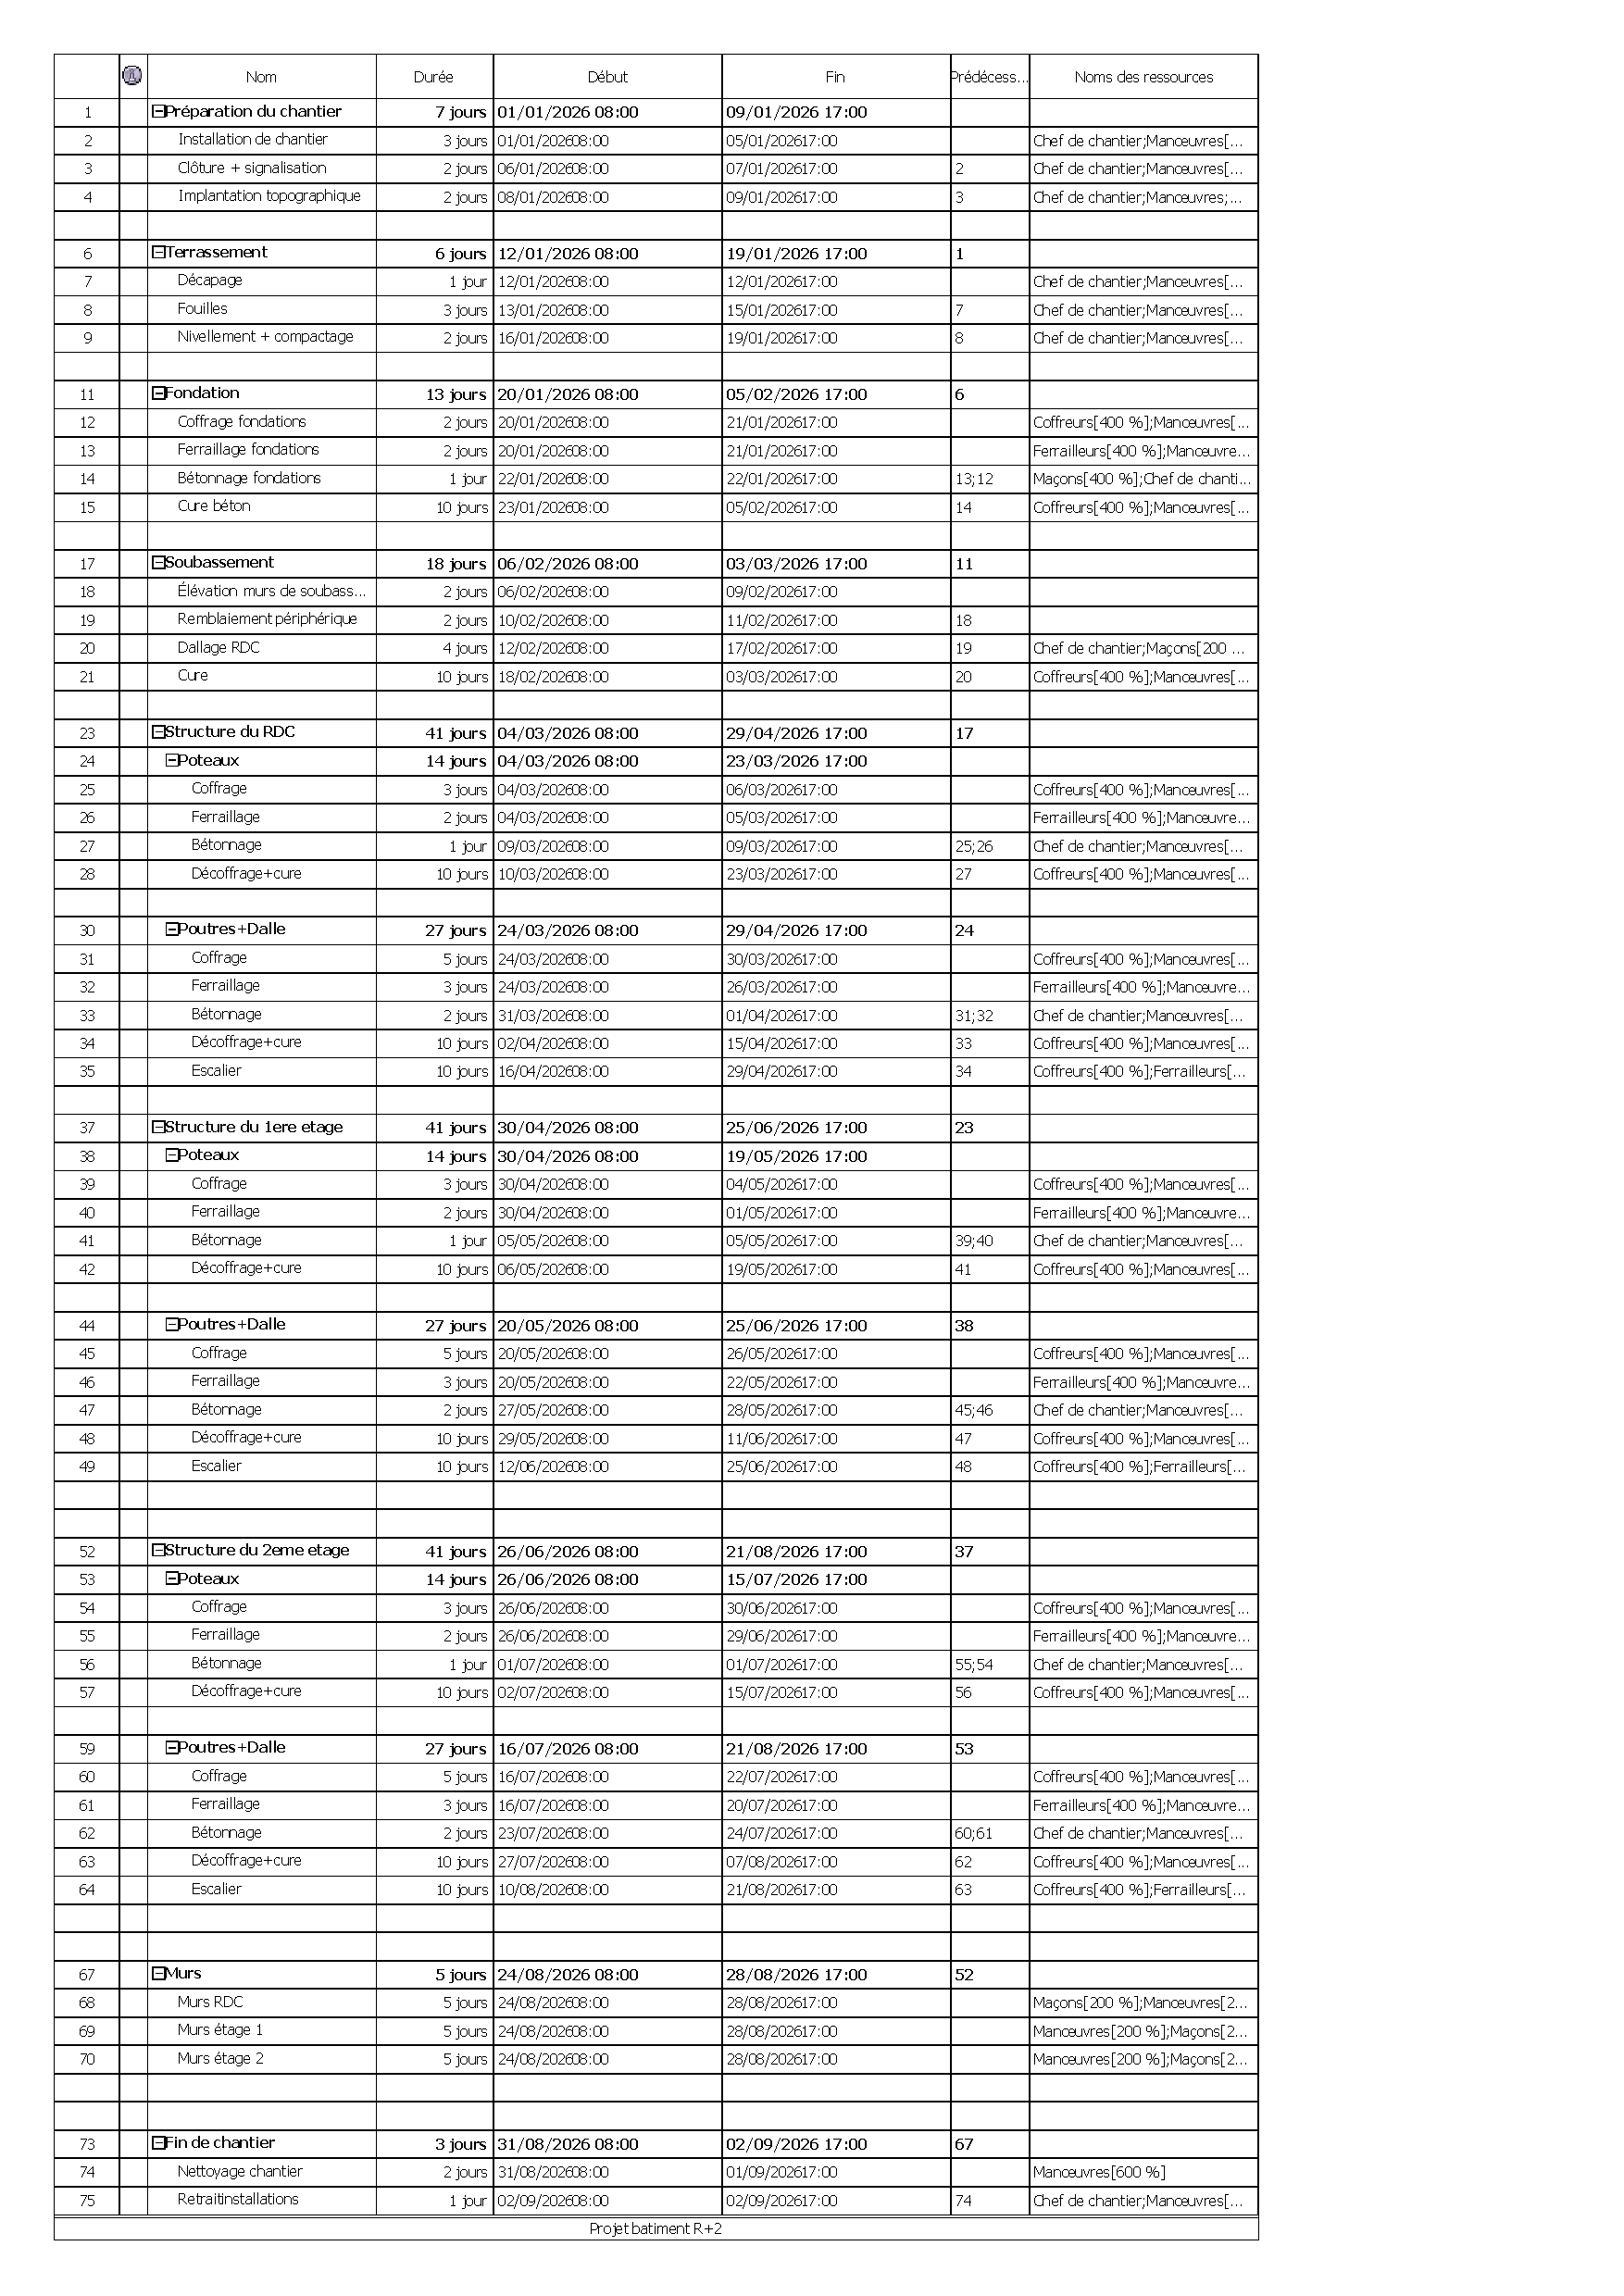
\includegraphics[width=1\linewidth]{tableau}
		\label{fig:tableau}
	\end{figure}
	
	\begin{figure}[H]
		\centering
		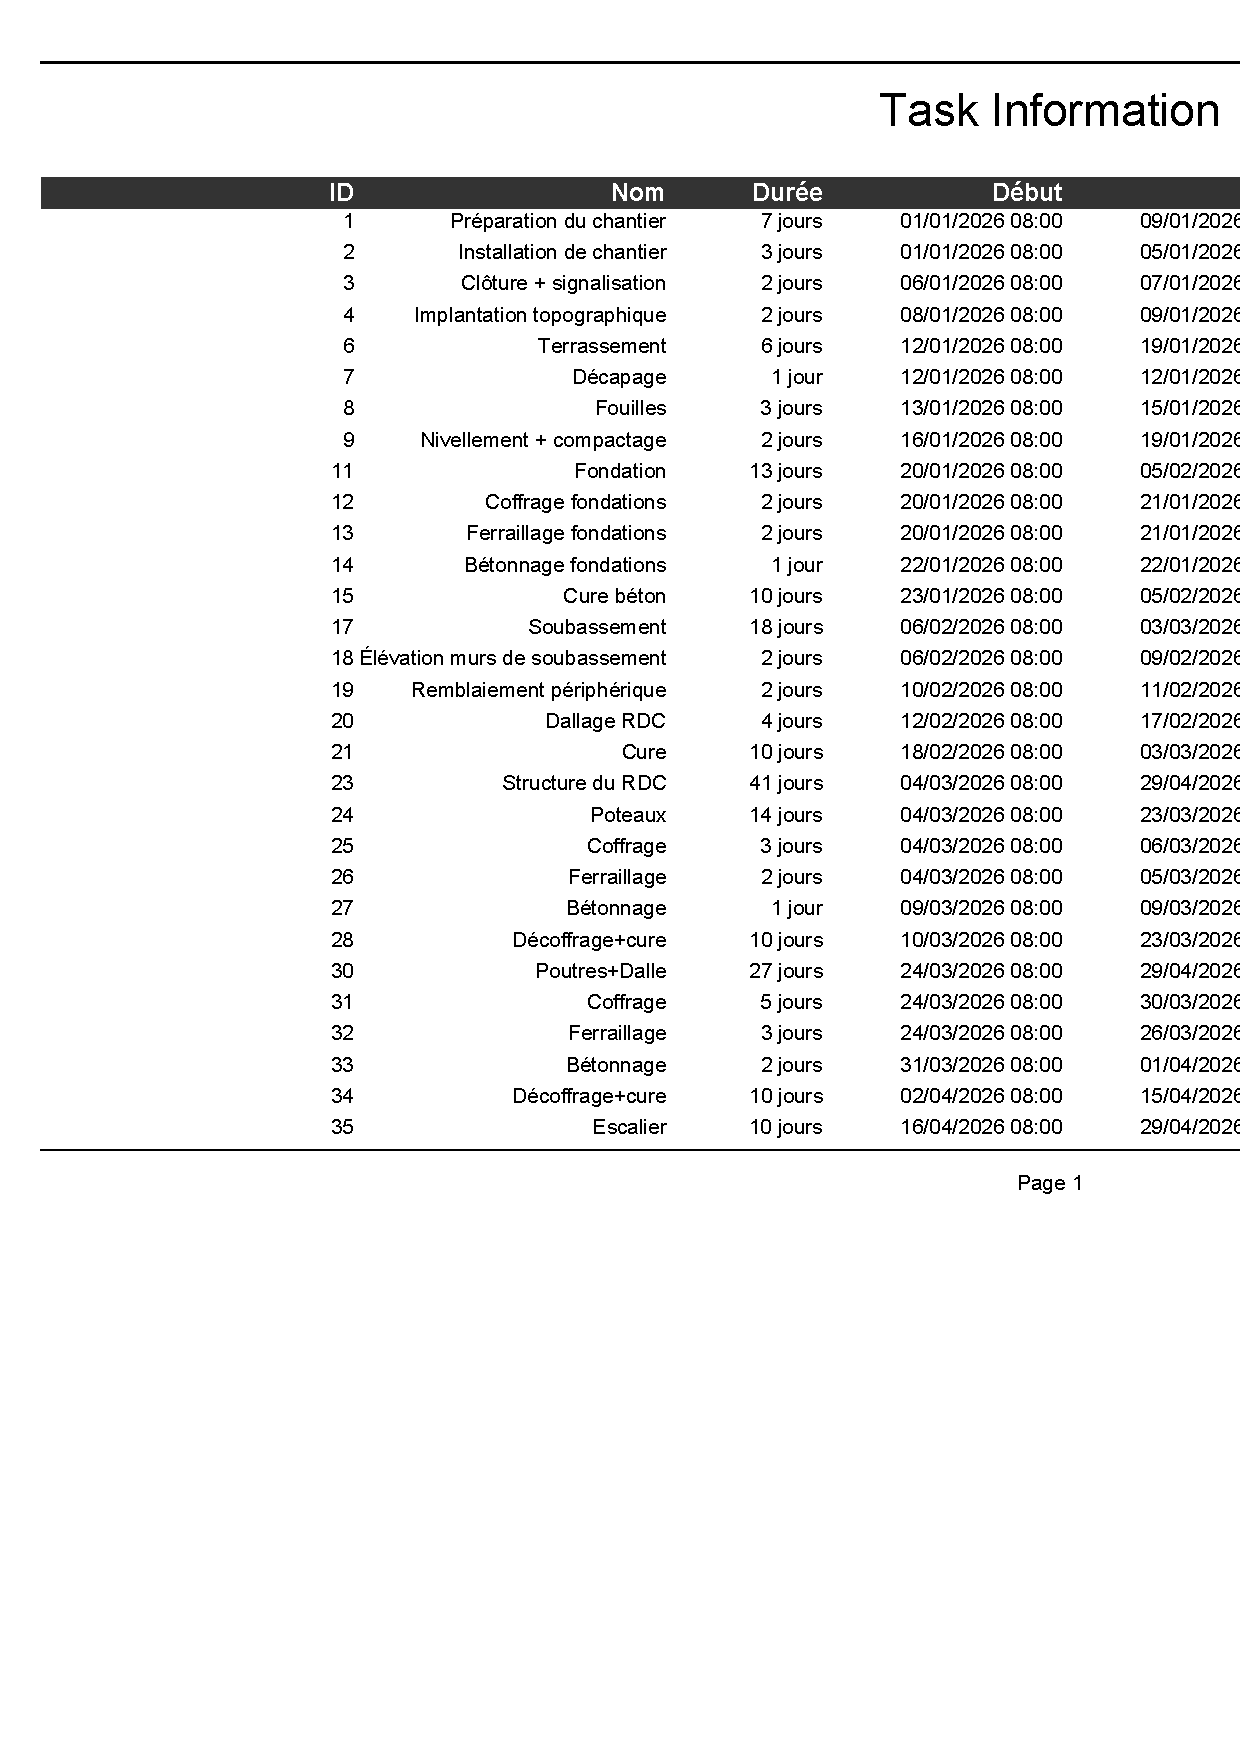
\includegraphics[width=1\linewidth]{task-dinar}
		\label{fig:task-dinar}
	\end{figure}
	
	
	\section{Ressources du projet}
	

	\begin{figure}[H]
		\centering
		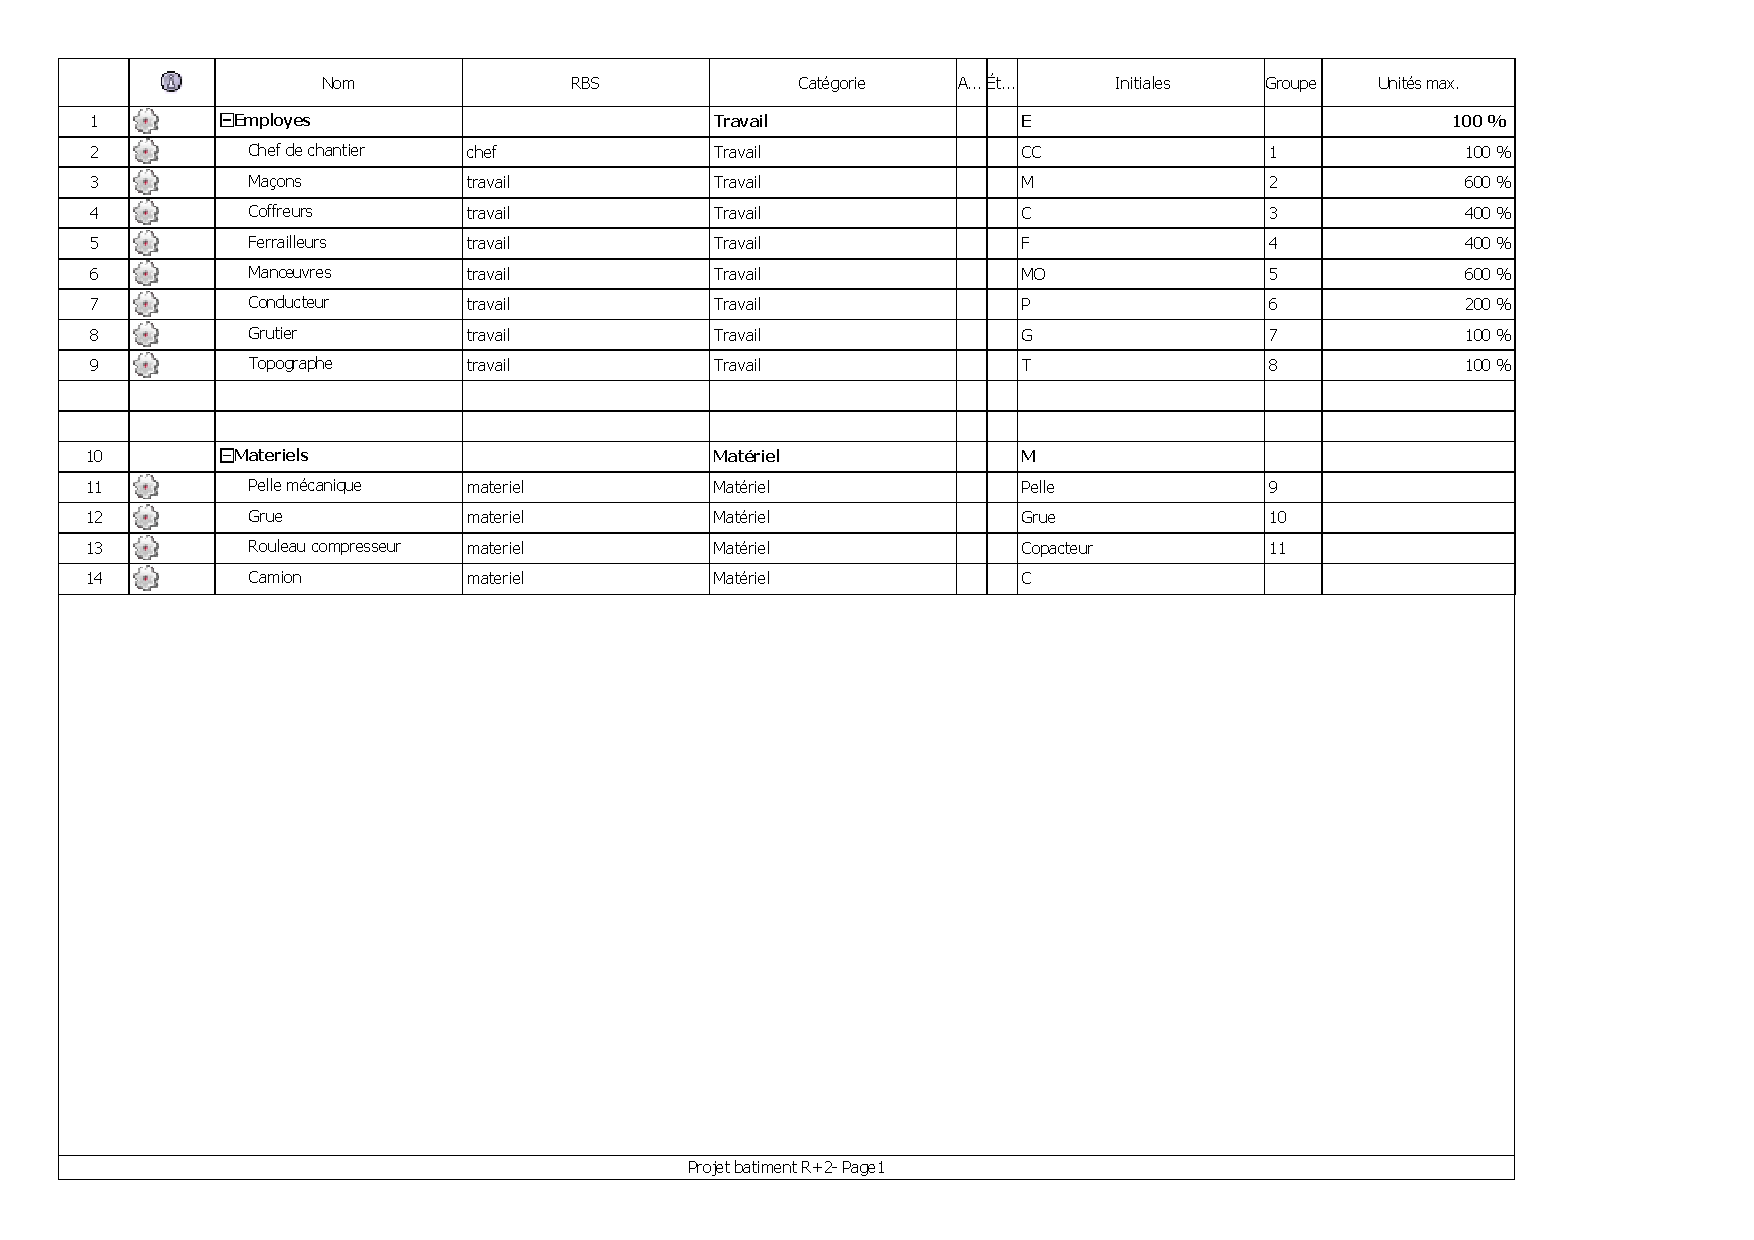
\includegraphics[width=1\linewidth]{ressources}
		\caption{Tableau des ressources}
		\label{fig:ressources}
	\end{figure}
	

	Pour le salaire des employés voir le fichier de ProjectLibre, leur salaire a été posé en dinars.
	
	
	
	

	
	\section{Planning général du chantier}
	
	Le planning général du projet a été élaboré à l’aide du logiciel
	\textbf{ProjectLibre}. Il présente l’enchaînement des tâches, leurs durées,
	les ressources affectées ainsi que le chemin critique.
	
	\vspace{\baselineskip}
	
	
	On peut voir que la durée du projet est estimer à 9 mois ou a 175 jours de travails net.
	
	\vspace{\baselineskip}
	
	On remarque aussi que toute les tâches sont critiques a l'exception des étapes de ferraillages qui se font en parallèle avec celle du coffrage, donc c'est uniquement à niveau qu'on peut ce permettre un retard sans affecter la durée du réalisation. 
	
	
	\section{Estimation des coûts}
	
	
	Uniquement le cout des ressources humaines a été pris en considération. (voir sur le fichier pour les estimations.)
	
	\vspace{\baselineskip}
	
	Le prix finale est de projet est de (salaire des employés uniquement) : 
	
	{\centering \textbf{\textcolor{red}{3 407 543,67 DA}}\par}
	
	Les détails seront joint dans des document PDF séparer ou bien voir le fichier .POD de PL.
	
	\section{Analyse du planning}
	
	L’analyse du planning permet de mettre en évidence :
	\begin{itemize}
		\item La durée totale du projet
		\item Les tâches critiques
		\item L’optimisation des ressources
	\end{itemize}
	
	Le respect de l’ordre d’exécution des travaux garantit la continuité du chantier
	et la maîtrise des délais.
	
	
	\section{Conclusion}
	
	Ce projet d’Organisation de Chantier a permis de mettre en application les notions théoriques, notamment la planification, la gestion des ressources et l’estimation des coûts. L’utilisation du logiciel ProjectLibre s’est révélée efficace pour structurer le projet, visualiser l’enchaînement des tâches et optimiser la durée globale du chantier.
	
	\vspace{\baselineskip}
	
	Ce travail constitue une base réaliste et cohérente pour la gestion d’un chantier de bâtiment de type R+2.
	
	
	
\end{document}